% Copyright (c) 2019-2021, Julien Seguinot (juseg.github.io), Ian Delaney
% Creative Commons Attribution-ShareAlike 4.0 International License
% (CC BY-SA 4.0, http://creativecommons.org/licenses/by-sa/4.0/)

% Alps erosion paper
% ==================

\documentclass[esurf, manuscript]{copernicus}
\usepackage{CJK}  % Japanese text

% custom colours (colorbrewer2.org)
\definecolor{Bu}{cmyk}{1.00,0.45,0.00,0.07}  % Blues
\definecolor{Gn}{cmyk}{1.00,0.20,1.00,0.00}  % Greens
\definecolor{Rd}{cmyk}{0.35,0.95,0.85,0.00}  % Reds
\definecolor{Or}{cmyk}{0.35,0.75,1.00,0.00}  % Oranges
\definecolor{Pu}{cmyk}{0.70,0.80,0.00,0.00}  % Purples
\definecolor{Br}{cmyk}{0.40,0.75,1.00,0.00}  % YlOrBr

% custom commands (remove before submission)
\newcommand{\note}[1]{\textcolor{Or}{\emph{[\textbf{NOTE:} #1]}}}
\newcommand{\todo}[1]{\textcolor{Rd}{\emph{[\textbf{TODO:} #1]}}}

% color links (remove before submission)
\hypersetup{colorlinks, citecolor=Bu, linkcolor=Bu, urlcolor=Bu}

% figures directory
\graphicspath{{../../figures/}}

% document properties
\title{Last glacial cycle glacier erosion potential in the Alps}
\Author[1]{Julien}{Seguinot}
\Author[2]{Ian}{Delaney}
\affil[1]{Independent scholar, Anafi, Greece}
\affil[2]{Institute of Earth Surface Dynamics, University of Lausanne, Switzerland}
\runningtitle{Last glacial cycle glacier erosion potential in the Alps}
\runningauthor{J.~Seguinot and I.~Delaney}


% ======================================================================
\begin{document}
% ======================================================================

\maketitle

\begin{abstract}

    The glacial landscape of the Alps has fascinated generations of explorers,
    artists, mountaineers and scientists with its diversity, including
    erosional features of all scales from high-mountain cirques, to steep
    glacial valleys and large over-deepened basins. Using previous glacier
    modelling results, and empirical inferences of bedrock erosion under modern
    glaciers, we compute a distribution of potential glacier erosion in the Alps
    over the last glacial cycle from 120\,000 years ago to the present.
    %
    Despite large uncertainties pertaining to the climate history of the Alps and
    unconstrained glacier erosion processes, the resulting modelled patterns of
    glacier erosion include persistent features. The cumulative imprint of
    the last glacial cycle shows a very strong localization of glacier erosion
    with local maxima at the mouths of major Alpine valleys and some other
    upstream sections where glaciers are modelled to have flown with the
    highest velocity. The modelled erosion rates vary significantly through the
    glacial cycle, but show paradoxically little relation to the total glacier
    volume. Phases of glacier advance and maximum extension see a localization
    of rapid erosion rates
    at low elevation, while glacier erosion at higher elevation is modelled
    date from phases of less extensive glaciation. The modelled erosion rates
    peak during deglaciation phases, when frontal retreat results in steeper
    glacier surface slopes, implying that climatic conditions that result in
    rapid glacier erosion might be quite transient and specific.
    %
    Our results depict the Alpine glacier erosion landscape as a
    time-transgressive patchwork, with different parts of the
    range corresponding to different glaciation stages and time
    periods.

\end{abstract}


% ----------------------------------------------------------------------
\introduction
% ----------------------------------------------------------------------

    \begin{figure*}[ht]
      \centerline{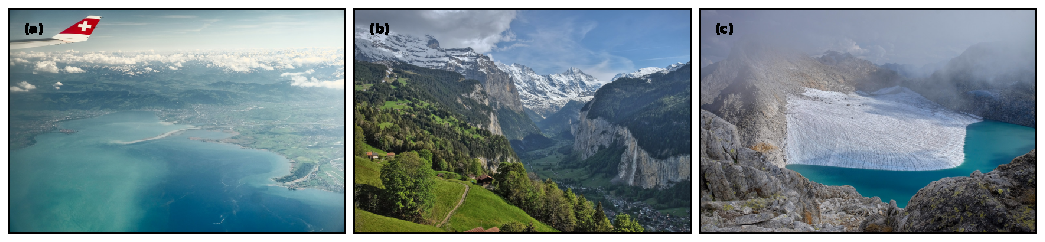
\includegraphics{alpero_landscape}}
      \caption{%
        Alpine glacial erosion landscape diversity.
        \textbf{(a)} Piedmont overdeepening of Lake Constance, ca.~10x50\,km.
        \textbf{(b)} Glacial trough of Lauterbrunnental, ca.~1x10\,km.
        \textbf{(c)} Mountain cirque of Ch\"uebodengletscher, ca.~1x1\,km.}
      \label{fig:landscape}
    \end{figure*}

    The glacial erosion landscape of the Alps has fascinated generations of
    explorers, artists, mountaineers and scientists for centuries. Its cultural
    impact is indeed so far-reaching, that in English, a non-Alpine language,
    the adjective ``alpine'' with non-capital ``a'' is now casually used to
    describe an Alpine-like, glacially modified mountain landscape outside the
    Alps, while the proper noun ``Alps'' has been applied to nick-name
    Alpine-like, glacier eroded mountain ranges in Norway (\emph{Lyngsalpene}),
    New Zealand (Southern Alps), Japan
    (\emph{\begin{CJK}{UTF8}{min}日本アルプス\end{CJK},
    Nihon Arupusu}), and elsewhere.
    %
    Some mountain ranges are predominantly characterised by cirque glaciation
    (e.g. Uinta Mountains), glacial valleys (e.g. Putorana Plateau), or
    large-scale overdeepenings (e.g. Patagonia). But other regions, including
    the Alps, present a higher variety of glacier erosional landforms
    \citep[][Fig.~\ref{fig:landscape}]{Ramsay.1862, Ball.1863, Gastaldi.1873,
    Penck.1905} whose implications on glacial history is yet to be understood.

    In absence of other landforms, glacially eroded topography has sometimes
    been used as a proxy for glacier extent, for instance in
    geomorphological mapping \citep[e.g.,][]{Margold.etal.2011, Fu.etal.2012}.
    Cold-based glaciers, however, have been observed to preserve landforms as
    fragile as sand beaches \citep{Kleman.1994}, leading to the
    reinterpretation of complex glacial landscapes within a binary conceptual
    framework of cold and temperate basal thermal regimes
    \citep{Kleman.etal.2008, Kleman.etal.2010, Fabel.etal.2012, Fu.etal.2013}.
    Nevertheless, it remains unclear how sharp the erosional
    transition to cold-based ice is, and why some glaciated regions show
    characteristic landform preservation and others, including the Alps, do not
    \citep{Wirsig.etal.2016, Seguinot.etal.2018}.

    Glacier erosion also likely governs, at least in part,
    the height of mountains \citep{Egholm.etal.2009,Thomson.etal.2010} through
    the ``glacier buzz-saw''. In turn, evidence suggests that increased
    mountain erosion rates coincided with global cooling and Pliestocene
    glaciations from roughly 2.6 million years before present
    \citep{Herman.Champagnac.2016}. Yet, oceanic isotopic proxies for global
    weathering rates remained constant over this time period
    \citep{Willenbring.Von-Blanckenburg.2010}. Examination of contemporary
    erosion rates across different climates suggest that increased temperatures
    in glaciated regions lead to higher erosion rates and that erosion rates
    may have increased towards present \citep{Koppes.Montgomery.2009,
    Koppes.etal.2015, Fernandez.etal.2016}. However, understanding the link
    between climate and glacier erosion in the sedimentary record remains
    difficult due to time scale biases \citep{Ganti.etal.2016} and the
    non-linear relationship  between atmospheric temperature and erosion
    \citep[e.g.,][]{Anderson.etal.2012,Mariotti.etal.2021}.

    Observing and quantifying the long-term glacier erosion and sedimentation
    processes has been a challenge, and two general methods have been adopted
    to quantify erosion \citep{Alley.etal.2019}. Physically-based models
    describe quarrying process and abrasion of bedrock by debris laden ice
    \citep[e.g.,][]{Alley.etal.1997, Iverson.2012, Beaud.etal.2014}. Describing
    the processes physically provides a basis for understanding erosion
    processes \citep{Hallet.1979, Ugelvig.etal.2018} and yields insight into
    the formation of glacial landforms, such as tunnel valleys and eskers
    \citep{Beaud.etal.2018, Hewitt.Creyts.2019}. Yet, these models prove
    difficult to implement in many cases due to the large number of poorly
    constrained parameters and process, i.e. water pressure fluctuations and
    subglacial debris concentration \citep[e.g.,][]{Hallet.1979, Seguinot.2008,
    Ugelvig.etal.2018}.

    Instead, empirical relationships between glacier sliding and erosion can
    represent erosional quantities well and can recreate important glacial
    landforms \citep[e.g.,][]{Harbor.etal.1988, Macgregor.etal.2000}.
    For instance, \citet{Humphrey.Raymond.1994} correlated temporal variations
    in ice velocity and suspended sediment load during a surge of Variegated
    Glacier to establish a linear erosion law.
    \citet{Koppes.etal.2015} quantified sediment
    yields in 15~Patagonian and Antarctic Peninsula fjords, concluding at a
    predominant control of surface air temperature on rapid glacier erosion and
    calibrating a near-square-law from glacier velocity to erosion rate.
    \citet{Herman.etal.2015} collected suspended sediment samples for 5~months
    in the outlet stream of Franz-Josef Glacier, mapped their chemical
    composition to geologic zones of distinctive glacier speed, and also
    concluded to a near-square relationship between basal sliding and glacier
    erosion.
    \citet{Cook.etal.2020} assembled a global compilation of erosion rates for
    38~glaciers, showing a predominant role of glacier sliding velocity over
    climate variables, yet concluding at a sub-linear relationship to erosion.

    Here, the non-linear erosion law by \citet{Koppes.etal.2015} is applied to
    previously published model results \citep{Seguinot.etal.2018} and the
    patterns of modelled erosion rates and cumulative last glacial cycle erosion
    potential are analysed. We examine the glaciological conditions that cause
    erosion and discuss the implications of these conditions on understanding
    the relationship between climate and glacier erosion. Despite aggregated
    uncertainties on paleoclimate, glacier flow and glacier erosion processes,
    out results provide insights into the diversity of the Alpine glacial
    erosion landscape.


% ----------------------------------------------------------------------
\section{Methods}
% ----------------------------------------------------------------------

% -- -- -- -- -- -- -- -- -- -- -- -- -- -- -- -- -- -- -- -- -- -- -- -
\subsection{Ice sheet modelling}
% -- -- -- -- -- -- -- -- -- -- -- -- -- -- -- -- -- -- -- -- -- -- -- -

    The ice-sheet model set-up was presented in an earlier publication
    \citep{Seguinot.etal.2018} and is briefly summarized here. The simulations
    were conducted using the Parallel Ice Sheet Model (PISM, development
    version~e9d2d1f), an open-source, finite-difference, shallow-ice and
    shallow-shelf model
    \citep{PISM-authors.2017}. Our setup includes temperature and water-content
    dependent creep, pseudo-plastic basal sliding accounting for till
    dilatation under high water pressure, bedrock deformation under the ice
    load, and a~positive degree-day (PDD) surface mass balance model. The model
    is initialized with assumed present-day ice thickness and equilibrium
    ice and bedrock temperature at 120\,ka (thousand years before the present),
    and ran to the present. The ice-sheet model physical parameters are listed
    in the earlier open-access publication \citep{Seguinot.etal.2018}, and the
    complete list of PISM
    parameters is stored in long-term archived model output metadata for the
    present study \citep{Seguinot.2021}, and for the earlier publication
    \citep{Seguinot.2020, Seguinot.2020a}.

    Climate forcing is provided by a~monthly climatology from interpolated
    observational data \citep[WorldClim;][]{Hijmans.etal.2005} and the European
    Centre for Medium-Range Weather Forecasts Reanalysis Interim
    \citep[ERA-Interim;][]{Dee.etal.2011}, amended with temperature lapse-rate
    corrections from the European Project for Ice Coring in Antarctica
    \citep[EPICA;][] {Jouzel.etal.2007}, and time-dependent paleo-precipitation
    reductions \citep{Huybrechts.2002}. Lower-resolution runs based on
    alternative paleoclimate scenarios \citep{Seguinot.etal.2018} are analyzed
    in the discussion part (Sect.~\ref{sec:sensitivity}).

% -- -- -- -- -- -- -- -- -- -- -- -- -- -- -- -- -- -- -- -- -- -- -- -
\subsection{Erosion law}
% -- -- -- -- -- -- -- -- -- -- -- -- -- -- -- -- -- -- -- -- -- -- -- -

    Modelled erosion rates, $\dot{e}$, are calculated from the modelled basal
    velocities, $u_\mathrm{b}$, using a empirical erosion power-law,
    %
    \begin{equation}
        \dot{e} = K_\mathrm{g} u_\mathrm{b}^l ,
    \end{equation}
    %
    where $K_g = 5.2\times 10^{-11}\,m^{1-l}\,a^{l-1}$ and $l = 2.34$ are
    empirical constants calibrated on quantified fjord sediment yields and
    velocities from 15~Patagonian and Antarctic Peninsula tidewater glaciers
    \citep{Koppes.etal.2015}. We discuss the role of alternative values of
    $K_\mathrm{g}$ and $l$ in the discussion part (Sect.~\ref{sec:powerlaws}).

    Our approach does not account for feedbacks of glacier erosion onto
    bedrock topography and, then onto, ice dynamics
    \citep[e.g.,][]{Anderson.etal.2012}. Furthermore, we assume that once
    material is eroded, it is transported out of the system. In turn, we do not
    account for the downstream advection of debris
    \citep[e.g.,][]{Anderson.Anderson.2016}, or fluvial transport of subglacial
    sediment \citep{Delaney.etal.2019}. Instead, we compute the
    time-integrated glacier erosion rate,
    %
    \begin{equation}
        e =  K_\mathrm{g} \int u_\mathrm{b}^l dt,
    \end{equation}
    %
    and refer to it as the cumulative ``erosion potential''. The integration
    is numerically approximated using a time-step of 10\,a in the
    main simulation, and 100\,a in the alternative climate scenarios runs.
    Note that in the above formula with an exponent, $l$,
    higher than one, the cumulative erosion potential has a greater dependency
    on the basal ice dynamics, $u_\mathrm{b}$, than the duration of glacier
    cover.


% ----------------------------------------------------------------------
\section{Results}
% ----------------------------------------------------------------------

% -- -- -- -- -- -- -- -- -- -- -- -- -- -- -- -- -- -- -- -- -- -- -- -
\subsection{Cumulative erosion}
% -- -- -- -- -- -- -- -- -- -- -- -- -- -- -- -- -- -- -- -- -- -- -- -

    \begin{figure*}[ht]
      \centerline{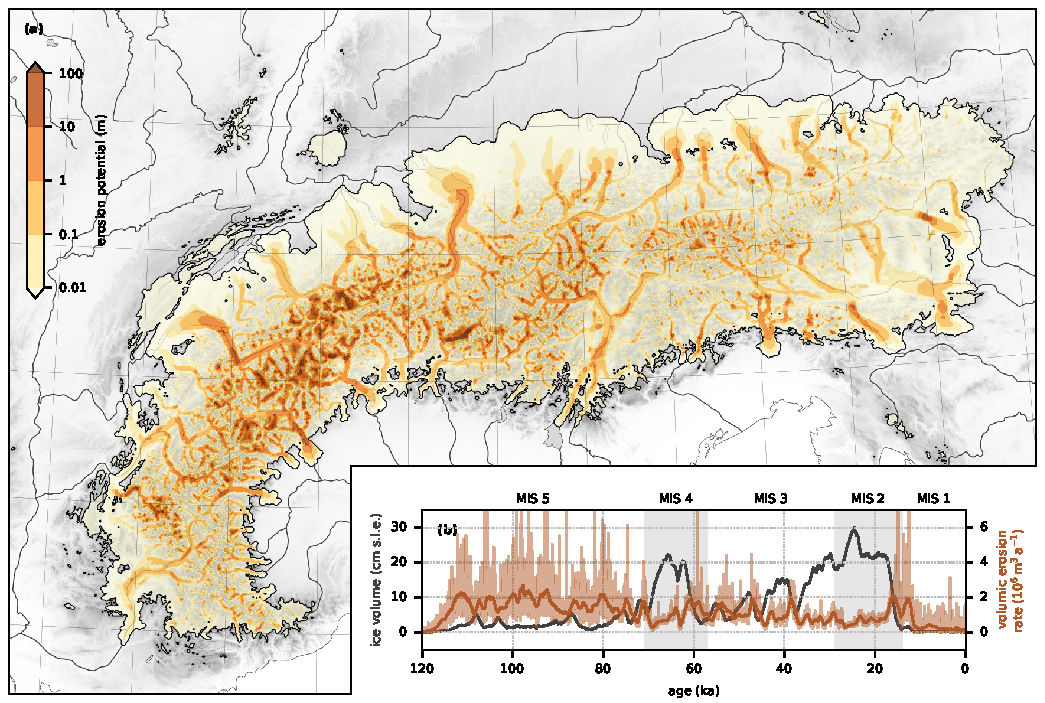
\includegraphics{alpero_cumulative}}
      \caption{%
        \textbf{(a)} Modelled cumulative (time-integrated) glacial erosion
          potential over the last glacial cycle.
        \textbf{(b)} Modelled total ice volume in centimetres of sea-level
          equivalent (cm~s.l.e., black), annual (domain-integrated) erosion
          volume (light brown) and 100-a running mean (dark brown). Shaded gray
          areas indicate the timing for MIS~2 and~4
          \citep{Lisiecki.Raymo.2005}.}
        \label{fig:cumulative}
    \end{figure*}

    The modelled cumulative (time-integrated) glacial erosion potential
    (Fig.~\ref{fig:cumulative}a) varies by several orders of magnitude
    from insignificant to hundred-metres-scale erosion potential. Its spatial
    patterns show a very strong localization along the Alpine valleys, with
    local maxima occurring both at
    the Alpine gates where ice flow transited from valley to piedmont glaciers,
    and further upstream where the valley slopes increase. While mountain
    cirques are poorly captured by the model's horizontal resolution, high
    cumulative erosion potential also occurs near the valley heads.
    There is a general tendency for higher cumulative erosion in the
    north-western Alps where the input winter precipitation is higher
    \citep[WorldClim, Fig.~1h in][]{Seguinot.etal.2018} and the glacial relief
    more pronounced in the topography.

% -- -- -- -- -- -- -- -- -- -- -- -- -- -- -- -- -- -- -- -- -- -- -- -
\subsection{Temporal evolution}
% -- -- -- -- -- -- -- -- -- -- -- -- -- -- -- -- -- -- -- -- -- -- -- -

    \begin{figure}[ht]
      \centerline{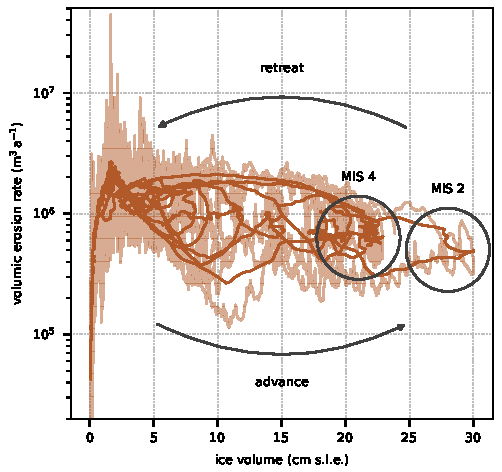
\includegraphics{alpero_evolution}}
      \caption{%
        Modelled annual (domain-integrated) erosion volume (light brown) and 100-a
        running mean (dark brown) in relation to modelled total ice volume in
        centimetres of sea-level equivalent.}
      \label{fig:evolution}
    \end{figure}

    The modelled annual (domain-integrated) glacial erosion volume
    does not systematically correlate with the modelled total ice volume
    (Fig.~\ref{fig:cumulative}b). Except for the onset and termination of the
    glacial cycle were ice volume is low and sliding processes unlikely to be
    captured by the model resolution, a comparison between the modelled ice
    volume and the modelled annual erosion volume shows no single relation
    between these two quantities (Fig.~\ref{fig:evolution}). After significant
    ice volume has been reached, there is a slight tendency for slower erosion
    during periods of extensive glaciation (Fig.~\ref{fig:evolution}). However,
    the domain-integrated erosion volume is modelled to be consistently higher
    (by a factor 2 to 10) during periods of decreasing ice volume, than during
    periods of increasing ice volume (Fig.~\ref{fig:evolution}).

% -- -- -- -- -- -- -- -- -- -- -- -- -- -- -- -- -- -- -- -- -- -- -- -
\subsection{Spatial migration}
% -- -- -- -- -- -- -- -- -- -- -- -- -- -- -- -- -- -- -- -- -- -- -- -

    \begin{figure*}[ht]
      \centerline{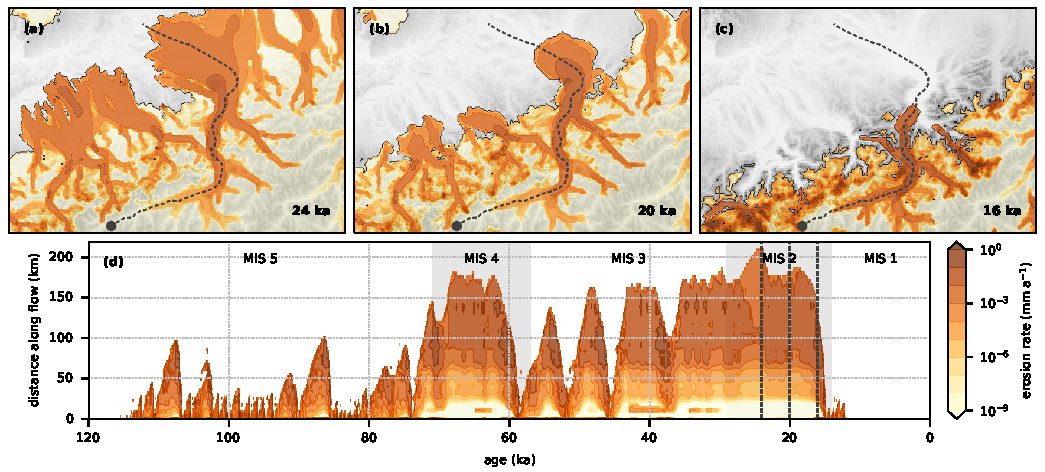
\includegraphics{alpero_transects}}
      \caption{%
        \textbf{(a, b, c)} Modelled instantaneous erosion rate of the Rhine
          Glacier for selected post-Last Glacial Maximum ages.
        \textbf{(d)} Interpolated instantaneous erosion rate along a Rhine
          Glacier transect for the entire last glacial cycle (upper panels
          dashed line).}
      \label{fig:transects}
    \end{figure*}

    \begin{figure*}[ht]
      \centerline{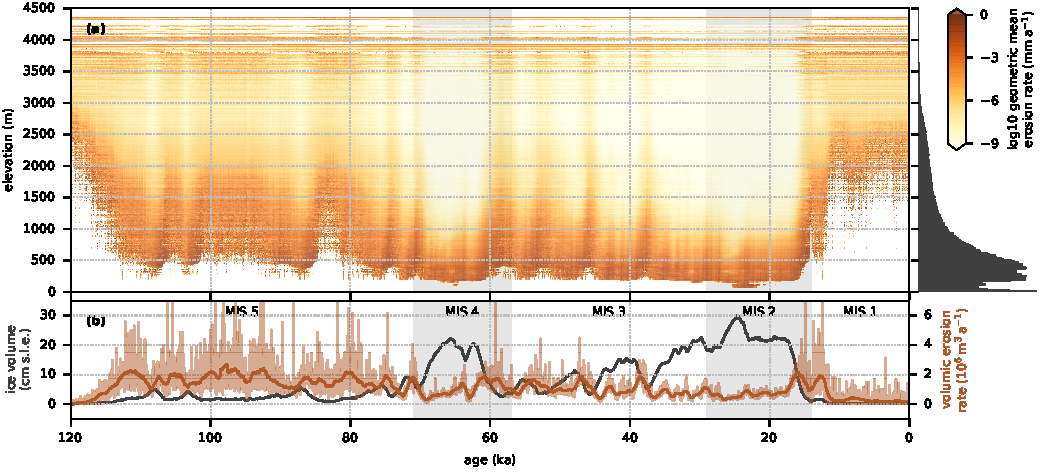
\includegraphics{alpero_hypsogram}}
      \caption{%
        \textbf{(a)} Modelled erosion rate ``hypsogram'', showing the geometric
          mean of (non-zero) modelled erosion rates in 10-m elevation bands
          across the entire model domain and its time evolution. The histogram
          to the side shows the distribution of topography in the model domain.
        \textbf{(b)} Same as Fig.~\ref{fig:cumulative}b.}
      \label{fig:hypsogram}
    \end{figure*}

    A closer look at the Rhine Glacier, one of the paleo-ice sheet's largest
    outlets, reveals a spatial migration of the modelled rapid erosion areas.
    During stages of glacier advance and maximum extension, erosion is modelled
    to be under 1\,mm\,a$^{-1}$ and restricted the lower parts of the
    catchment, while much the intra-montane Alps \citep[modelled to be largely
    cold-based, Fig.~6c in][]{Seguinot.etal.2018}, experience
    insignificant erosion (Fig.~\ref{fig:transects}a and~d). The modelled
    erosion rates both increase and propagate inwards during periods of glacier
    retreat (Fig.~\ref{fig:transects}b, c and~d).

    The results found on the Rhine Glacier catchment can be generalized to the
    entire model domain by using (present-day) bedrock altitude as a proxy for
    along-flow distance (Fig.~\ref{fig:hypsogram}). Thus more generally,
    periods of modelled increasing and maximum ice volume correspond to lower
    values for elevation-aggregated erosion rates, with significant erosion
    restricted to lower elevations. On the opposite, periods of modelled
    decreased ice volume correspond to higher local modelled erosion rates and
    more extensive rapid erosion into higher-elevation areas
    (Fig.~\ref{fig:hypsogram}).


% ----------------------------------------------------------------------
\section{Discussion}
% ----------------------------------------------------------------------

% -- -- -- -- -- -- -- -- -- -- -- -- -- -- -- -- -- -- -- -- -- -- -- -
\subsection{Climate sensitivity}
\label{sec:sensitivity}
% -- -- -- -- -- -- -- -- -- -- -- -- -- -- -- -- -- -- -- -- -- -- -- -

    \begin{figure*}[ht]
      \centerline{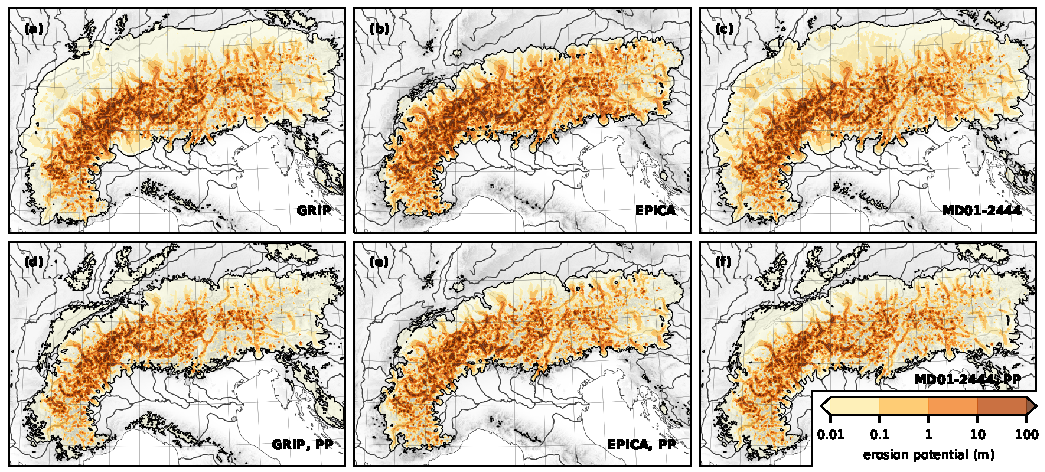
\includegraphics{alpero_sensitivity}}
      \caption{%
        Modelled cumulative glacial erosion potential over the last glacial
        cycle without \textbf{(a, b, c)} and with \textbf{(d, e, f)}
        paleo-precipitation corrections, and using three different
        palaeo-temperature histories \citep[see][]{Seguinot.etal.2018}.}
      \label{fig:sensitivity}
    \end{figure*}

    Different paleoclimate forcing scenarios lead to different modelled
    glaciation histories \citep[cf.][]{Seguinot.etal.2018} and thus different
    results in terms of erosion
    potential (Fig.~\ref{fig:sensitivity}). Scenarios including higher
    (constant, present-day) input precipitation rates yield generally higher
    modelled
    erosion potential (Fig.~\ref{fig:sensitivity}a, b, and~c), while scenarios
    including paleo-precipitation reductions (Fig.~\ref{fig:sensitivity}d, e,
    and~f), including our default high-resolution run
    (Fig.~\ref{fig:cumulative}), yield a smaller erosion potential. The spatial
    pattern of modelled time-integrated erosion is nevertheless generally
    consistent across the paleoclimate scenarios tested,
    despite variations in the glaciation maximum extent
    (\citealp[Fig.~3 in][]{Seguinot.etal.2018}; Fig.~\ref{fig:sensitivity}).
    Furthermore, these changes are minor
    considering the large uncertainties affecting the choice of erosion law.

% -- -- -- -- -- -- -- -- -- -- -- -- -- -- -- -- -- -- -- -- -- -- -- -
\subsection{Choice of erosion law}
\label{sec:powerlaws}
% -- -- -- -- -- -- -- -- -- -- -- -- -- -- -- -- -- -- -- -- -- -- -- -

    \begin{figure*}[ht]
      \centerline{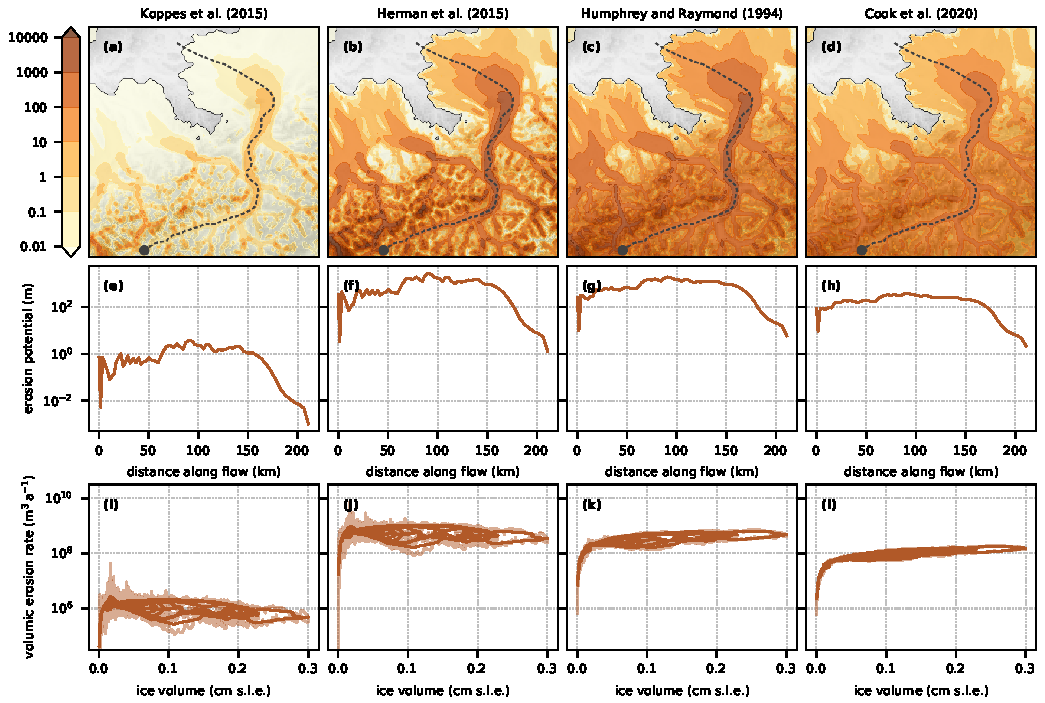
\includegraphics{alpero_powerlaws}}
      \caption{%
        Modelled cumulative (time-integrated) glacial erosion potential for
        three different erosion laws published by
        \textbf{(a)} \citet{Koppes.etal.2015},
          ${5.2 \times 10^{-8} u_\mathrm{b}^{2.34}}$ (same as
          Fig.~\ref{fig:cumulative}a but with a different colour scale),
        \textbf{(b)} \citet{Herman.etal.2015},
          ${2.7 \times 10^{-7} u_\mathrm{b}^{2.02}}$,
        \textbf{(c)} \citet{Humphrey.Raymond.1994},
          ${1 \times 10^{-4} u_\mathrm{b}^{1}}$, and
        \textbf{(d)} \citet{Cook.etal.2020},
          ${1.665 \times 10^{-1} u_\mathrm{b}^{0.6459}}$.
        \textbf{(e-h)} Corresponding modelled cumulative glacial erosion
          potential along a Rhine Glacier transect (upper panels dashed line), and
        \textbf{(i-l)} corresponding modelled evolution of annual
        (domain-integrated) erosion volume (light brown) and 100-a
        running mean (dark brown) in relation to modelled total ice volume in
        centimetres of sea-level equivalent (as in Fig.~\ref{fig:evolution}a).}
      \label{fig:powerlaws}
    \end{figure*}

    The choice of erosion law significantly impacts the results
    (Fig.~\ref{fig:powerlaws}). Our default, based on quantified
    sediment yields from Patagonian and Antarctic Peninsula tidewater glaciers
    \citep[${\dot{e}=5.2\times10^{-8}u_\mathrm{b}^{2.34}}$,][]{Koppes.etal.2015}
    yields a moderate and strongly localized cumulative erosion potential
    (Figs~\ref{fig:cumulative} and~\ref{fig:powerlaws}a). The erosion law
    based on measured suspended sediment load from Franz-Joseph Glacier
    \citep[${\dot{e}=2.7\times10^{-7}u_\mathrm{b}^{2.02}}$,][]{Herman.etal.2015}
    also yields a strongly localized, and yet much higher, modelled erosion
    potential (Fig.~\ref{fig:powerlaws}b). The erosion law based on measured
    suspended sediment load during a surge of Variegated Glacier
    \citep[${\dot{e}=1\times10^{-4}u_\mathrm{b}^{1}}$,][]{Humphrey.Raymond.1994}
    results in similarly high values, but a less localized pattern of cumulative
    erosion potential (Fig.~\ref{fig:powerlaws}c). Finally, The erosion law
    based on a global compilation of glacier velocities and erosion rates
    \citep[${\dot{e}=1.665\times10^{-1}u_\mathrm{b}^{0.6459}}$,][]{Cook.etal.2020}
    yields an even flatter pattern of cumulative erosion potential
    (Fig.~\ref{fig:powerlaws}d).

    It may seem surprising that the erosion law calibrated on Patagonian and
    Antarctic Peninsula tidewater glaciers \citep{Koppes.etal.2015} yields a
    more realistic glacial cycle erosion potential in the Alps than those based
    on terrestrial
    glaciers \citep{Humphrey.Raymond.1994, Herman.etal.2015, Cook.etal.2020},
    themselves resulting in kilometre-scale integrated erosion even
    higher than the Alpine relief itself. However, during the Last Glacial
    Maximum and much of the last glacial cycle, Alpine paleoglaciers were
    closer in size, slope, and climatic context to the present-day glaciers of
    Patagonia and the Antarctic Peninsula \citep{Koppes.etal.2015} than to
    Franz-Joseph Glacier \citep{Herman.etal.2015} and many of the glaciers
    included in the global compilation by \citet{Cook.etal.2020}. Indeed,
    atmospheric
    temperatures have been found to be a strong driver of erosion in studies
    involving several glaciers \citep{Koppes.etal.2015, Cook.etal.2020}.

    That said, the magnitude of the modelled erosion rates can hardly be used
    as a criteria to rule out this or that erosion law for the glacial Alps.
    While sliding is here modelled by a pseudo-plastic law based on
    till dilatation under high water pressure \citep{Tulaczyk.etal.2000},
    empirical erosion rules are thought to be a proxy for glacier abrasion
    (cf.~\citealp{Hallet.1979}; and possibly plucking) of a glacier flowing
    over a hard bed. Current erosion rates in the Alps strongly vary depending
    on the substratum \citep{Steinemann.etal.2020, Steinemann.etal.2021}, and
    it arguable that a layer of till and proglacial sediments may have armored
    the glacier bed from erosion for at least parts of the glacial cycle.
    Given the lack of data to constrain the erosion rule, it can not
    be excluded that a linear or sub-linear erosion-law
    \citep[e.g.,][]{Cook.etal.2020} would lead to a less localized pattern of
    erosion (Fig.~\ref{fig:powerlaws}c and~d), and a stronger correlation
    between modelled ice volume and erosion (Fig.~\ref{fig:powerlaws}k and~l).
    Even then, the intrinsically large variations in modelled glacier sliding
    velocities yield cumulative glacial-cycle erosion two to three orders of
    magnitude higher in the Alpine valleys than near the mountain tops
    (Fig.~\ref{fig:powerlaws}d).


% -- -- -- -- -- -- -- -- -- -- -- -- -- -- -- -- -- -- -- -- -- -- -- -
\subsection{Climate control on erosion}
% -- -- -- -- -- -- -- -- -- -- -- -- -- -- -- -- -- -- -- -- -- -- -- -

    \begin{figure}[ht]
      \centerline{\includegraphics{alpero_basaldrag}}
      \caption{%
        \textbf{(a)} Modelled basal and surface topographies interpolated along
        Rhine Glacier (using the same transect and ages as in
        Fig.~\ref{fig:basaldrag}).
        \textbf{(b)} Interpolated yield stress in the pseudo-plastic sliding law
        (dottel lines) and magnitude of the basal shear stress (basal drag,
        solid lines), both normalized against the ice overburden pressure
        \citep[cf.][for model physics]{Seguinot.2014, Seguinot.etal.2016}.}
      \label{fig:basaldrag}
    \end{figure}

    The modelled, domain-integrated glacier erosion volume do not increase
    together with ice volume. On the opposite, periods of ice advance and
    maximum glaciation correspond to comparatively slow erosion
    (Figs.~\ref{fig:cumulative} and~\ref{fig:evolution}).
    This result may seem paradoxical, and is modulated in a limited extent by
    the exponent, $l$, in the erosion rule (Fig.~\ref{fig:powerlaws}).
    During deglaciation periods, increased surface melt at low elevations
    results in a steepened topographic profile (Figs.~\ref{fig:basaldrag}a).
    The buttress formed by the glacier foot against gravitational forces is
    reduced, causing an increase in the magnitude of the basal shear stress
    (basal drag) relative to the ice overburden pressure, and an increase in
    the area where sliding and thus, erosion, can occur
    (Figs.~\ref{fig:basaldrag}b).

    This result is corroborated by a recent denudation record from the
    Mediterranean Alps, which includes an increase in glacier erosion in the
    Var Valley, roughly at 25\,ka following an extended period of low
    denudation rates \citep{Mariotti.etal.2021}. While that increase in
    erosion predates the increase observed in our study (ca.~15\,ka;
    Fig.~\ref{fig:evolution}), it demonstrates that climatic conditions
    over-which glacier erosion occurs are relatively specific and likely
    transient. Other field-based studies have evidenced increased glacier
    erosion and pro-glacial sedimentation during the current deglaciation period
    \citep[e.g.,][]{Koppes.Montgomery.2009, Micheletti.Lane.2016,
    Lane.etal.2017, Bendixen.etal.2017}. Yet this increase has often been
    attributed to higher meltwater availability, promoting sediment transport
    \citep{Delaney.Adhikari.2020}, enhanced glacier sliding
    \citep{Herman.etal.2011}, and hydrofracturing, i.e.~plucking
    \citep{Hallet.1996, Ugelvig.etal.2018, Hildes.etal.2004}.

    But importantly, these hydrological processes are not included in our
    model, so that deglaciation surface meltwater is assumed to instantly exit
    the glacier with no effect on glacier dynamics \citep[cf.][for comparison]
    {Werder.etal.2013, Iverson.2012, Ugelvig.etal.2018}. The enhanced glacier
    velocity during periods of ice retreat is here modelled to result from
    changes in glacier geometry alone (Figs.~\ref{fig:basaldrag}b).
    Observed feedbacks between
    surface meltwater and basal sliding, not included in the model, presumably
    further accelerated erosion during deglaciation \citep{Herman.etal.2011}.
    Furthermore, we omit the fluvial transport of sediment, which could well
    increase sediment discharge and erosion with increased melt, so long as
    additional sediment remains available \citep{Delaney.Adhikari.2020}. Rapid
    glacier erosion can be expected to accompany the ongoing 21st-century
    deglaciation, especially for the ice sheets of Greenland and
    Antarctica where polythermal and cold-based glaciers are warming and
    sliding may increase \citep[e.g.,][]{Moon.etal.2012, Mouginot.etal.2014,
    Overeem.etal.2017}.

% -- -- -- -- -- -- -- -- -- -- -- -- -- -- -- -- -- -- -- -- -- -- -- -
\subsection{Age of the glacial landscape}
% -- -- -- -- -- -- -- -- -- -- -- -- -- -- -- -- -- -- -- -- -- -- -- -

    In many places throughout the Alps, significant modelled cumulative erosion
    occurs far inside the Alpine valleys (Fig.~\ref{fig:cumulative}). Yet
    instantaneous erosion rates show a time-transgressive radial pattern
    (Fig.~\ref{fig:transects}), so that high-altitude rapid erosion is not
    modelled to date from expansive glaciation stages, but instead to stages of
    intermediate glacier cover
    \citep[Fig.~\ref{fig:hypsogram};][]{Barr.etal.2019}.

    For instance, low-elevation piedmont over-deepened basins such as Lake
    Constance (Fig.~\ref{fig:landscape}), Lake Geneva and Lake Maggiore, are
    here modelled to be the product of extensive, Last Glacial Maximum-like
    glaciations. Other modeling work suggests that features such as these
    likely form when water can access the glacier bed and encourage glacier
    sliding and, thus, erosion \citep{Herman.etal.2011}. The model herein does
    not include subglacial hydrology, yet the role of climate warming to
    increasing glacier erosion to the lower elevations remains evident
    (Fig.~\ref{fig:hypsogram}).
    Alpine terrain with elevations above 1000\,m are modelled to
    experience virtually no erosion from 35 to 18\,ka BP
    (Fig.~\ref{fig:hypsogram}), so that many of the most spectacular,
    intermediate-elevation glacial valleys of the Alps as Lauterbrunnental
    (Fig.~\ref{fig:landscape}), Haslital (Upper Aare) or Bout du Monde (Upper
    Giffre) would date from periods of intermediate glacier extension.
    While the validity of the model results at high elevation are
    limited by the 1-km resolution and the shallow-ice physics
    \citep{Imhof.etal.2019}, the lack of rapid erosion at high-elevations for much
    of the modelled glacial cycle implies that the numerous Alpine mountain
    cirques such as Ch\"uebodensee (Fig.~\ref{fig:landscape}) would have formed
    over interglacial periods, when glaciers are confined to their cirques
    \citep{Barr.etal.2017, Barr.etal.2019}. Similar processes also occur on
    Himalayan glaciers and may limit erosion for the high elevation portion of
    that mountain range during cold periods as well, failing to offset uplift
    rates \citep{Harper.Humphrey.2003}.

    Finally, the time-transgressive nature of the modelled glacial erosion
    rates hint at a new explanation for the Alpine glacier trim-line and lack
    of cold-based glaciation evidence. Due to their geographic location in the
    mid-latitudes, and their steep topographic gradient, the Alps appear as a
    mountain range that hosted glaciers of various sizes throughout the varying
    climate of the Quaternary, resulting in a transgressive localization of
    glacier erosion throughout their elevational range, from the piedmont
    during glacial maxima, to the highest cirques during interglacial periods.
    The Alpine trim-line, in this case, would neither correspond to the upper
    reach of the Last Glacial Maximum glaciers \citep[e.g.,][]{Kelly.etal.2004},
    nor to an englacial temperate-ice boundary \citep{Coutterand.2010,
    Seguinot.etal.2018}, but to a time-transgressive upper limit of erosion from
    retreating glaciers on steep terrain.


% ----------------------------------------------------------------------
\conclusions
% ----------------------------------------------------------------------

    Due to compounded uncertainties regarding paleoclimate, glacier sliding and
    erosion processes, our quantitative results are very likely inaccurate.
    Yet, we draw the following qualitative conclusions:
    \begin{itemize}
      \item The non-linear physics of glacier deformation and sliding, combined
        with non-linear empirical erosion laws, results in a very strong
        localization of rapid glacier erosion in regions of fast flow.
      \item This high spatio-temporal variability hints at a complex
        relationship between climate and glacier erosion, so that a highly
        variable response of glacier erosion to climate should be expected.
      \item Increased gravitational drag due to surface profile steepening
        provide a mechanism
        for accelerated erosion during deglaciation periods, irrespective of
        surface meltwater penetration to the glacier bed.
      \item If a non-linear glacier erosion law is used, the climate-induced
        slowdown of erosion counterbalances glacier expansion, so that
        Alpine-wide glacier erosion volumes do not correlate with the ice volume.
      \item Rapid glacier erosion is restricted to low elevation during stages
        of glacier advance and maximum glaciation, but propagates up-valley to
        higher elevations during periods of glacier retreat.
      \item The diversity of the Alpine glacier erosion landscape appears to
        be the time-transgressive signature of a variety of glacial stages
        ranging from pan-Alpine ice sheets to modern-style mountain glaciers.
    \end{itemize}


% ----------------------------------------------------------------------
% Acknowledgements
% ----------------------------------------------------------------------

\codedataavailability{%
    PISM is available as open-source software (http://pism-docs.org).
    Time and domain-aggregated erosion variables such as used in the figures is
    available for the four presented erosion power-laws
    (\doi{10.5281/zenodo.4495419}). Other model output variables were
    previously made available (\doi{10.5281/zenodo.1423160},
    \doi{10.5281/zenodo.1423176}).}

\videosupplement{
    A supplementary animation is available
    (\url{https://vimeo.com/503162771}).}

\authorcontribution{%
    J.~Seguinot performed the computations and prepared the figures.
    I.~Delaney interpreted the results in a broader context. Both authors
    contributed to the text.}

\competinginterests{%
    The authors declare that they have no conflict of interest.}

\begin{acknowledgements}
    We are very thankful to Constantine Khroulev, Ed Bueler, and Andy
    Aschwanden for their constant help and development with PISM, without whom
    this work would not have been possible. J.~Seguinot would like to thank
    John Jansen and Martin Margold for insightful early discussions, Susan
    Ivy-Ochs for being a constant (droid) motivator, as well as Popi, Karsta
    and Stefan for welcoming him on Anafi and providing agreeable conditions
    for work in times of pandemic.
    J.~Seguinot exclusively used gear transported on a bike for 5000\,km across
    Europe and fourteen countries (except for new underwear).
    I.~Delaney thanks Fr\'ed\'eric Herman for valuable support and
    conversations while at University of Lausanne.
    The (previously published) ice flow simulations were made with computer
    resources provided by the Swiss National Supercomputing Centre (CSCS)
    allocations no.~s573 and sm13 to J.~Seguinot.
\end{acknowledgements}


% ----------------------------------------------------------------------
% References
% ----------------------------------------------------------------------

\bibliographystyle{copernicus}
\bibliography{../../../references/references}


% ======================================================================
\end{document}
% ======================================================================
